
\chapter{Results\label{cha:chapter3}}
\noindent
\indent To investigate the mechanism behind the effect of serotonin stimulation in mice during anaesthesia, a dynamic firing rate model was implemented, which simulates a simplified network of the mouse brain. Each brain area was modelled using a local excitatory-inhibitory (EI) circuit consisting of one E, one I population, and a mechanism controlling for adaptation (A) of the excitatory population. The implementation was guided by the EI network model proposed by Jercog et al. \cite{jercogUPDOWNCorticalDynamics2017}, who showed that this model produces UP and DOWN states similar to the UP and DOWN states that were observed in recordings from mice during anaesthesia \cite{ruiz-mejiasSlowFastRhythms2011}.

\section{Replication of mouse brain dynamics in an anaesthetic state\label{sec:prereq}}

\subsection{UP and DOWN states}
\noindent
\indent The model was able to reproduce the slow-wave oscillations that were observed during anaesthesia in previous experiments. Figure \ref{fig:UPDOWNstates} shows the results of a simulated session using the connected network model. Certain areas showed periods of high (UP) and low (DOWN) activity in the firing rate of the E and I populations. The frequency of the UP and DOWN states cycle was around 0.5-1Hz, which simulates the frequency of the UP-DOWN dynamics observed in the experimental data (Meijer et al., in preparation). The connections between the 14 areas on the figure were formed with a coupling strength of $G=2$, to ensure that the UP-DOWN dynamics were synchronous across regions (more about synchrony in section \ref{sec:synchronyresults} and Figure \ref{fig:synchrony}). The slow-wave oscillations occurred without any serotonin interference, as this simulation did not include the stimulation by serotonin. 

\begin{figure}[h]
    \centering
    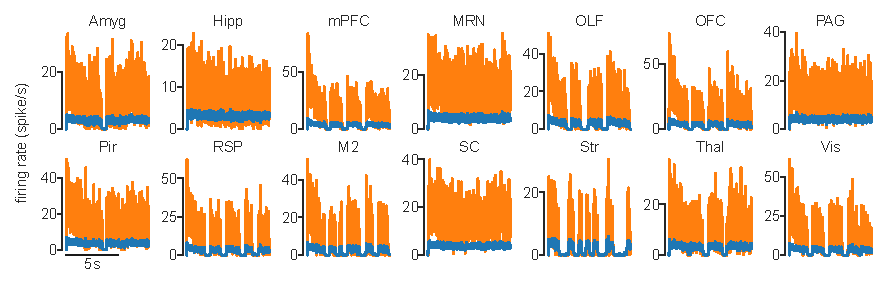
\includegraphics[width=1\textwidth]{img/Results/heterogeneous_UP-DOWN_states_S0_G2.pdf}
    \caption[Replication of UP and DOWN state dynamics]{Replication of UP and DOWN state dynamics. The 14 areas are connected via excitatory long-range projections. Without any serotonin stimulation, the activity in the brain regions is alternating between states of low and high activity, also named UP and DOWN states. The network is a heterogeneous network, accommodating the fact that not all areas show UP and DOWN states during anaesthesia.}
    \label{fig:UPDOWNstates}
\end{figure}

\subsection{Heterogeneity in the global circuit}\label{sec:heterogresults}

\noindent
\indent In the electrophysiological recordings it was observed that the UP-DOWN dynamics differed across brain regions. The hippocampus and midbrain areas clearly showed no state activity patterns, whereas cortical areas and the striatum clearly showed UP and DOWN states. The amygdala, thalamus and piriform showed less clear UP and DOWN states.
Adjusting the theta and beta parameter allowed for modification of the frequency of the UP-DOWN dynamics. This enabled introducing heterogeneity in the global network model making the simulation as close as possible to the experimental data. For example, in Figure \ref{fig:UPDOWNstates} the hippocampus only showed an UP state for the entire duration of the model simulation. This replicates the findings from the electrophysiological data and could be reached by setting the adaptation value to $\beta = 0$ and $\theta_E = 5$.  

\begin{figure}[h]
    \centering
    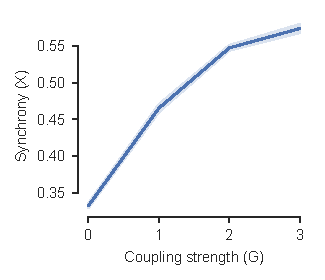
\includegraphics[width=0.45\textwidth]{img/Results/network_synchrony_brunelX.pdf}
    \caption{Synchrony in the global network model}
    \label{fig:synchrony}
\end{figure}

\subsection{Synchrony in the connected global network}\label{sec:synchronyresults}
\noindent
\indent The UP-DOWN dynamics that were visible during anaesthesia occurred in a synchronous rhythmic pattern. To evaluate the amount of synchrony in the network model, a measure proposed by Brunel and Hansel \cite{brunelCommunicatedPaulTiesinga2006} was applied (see Section \ref{cha:brunel} for methodological details). Running the model simulation using different coupling strength values tests
if the model follows this mechanism. Increasing the coupling strength increased the synchrony of the firing rates across the regions of the network. Since some of the areas did not show any UP and DOWN states, full synchrony ($\chi=1$) is not possible to reach. If not otherwise specified, $G=2$ was used in the following stimulation, corresponding to a value of $\chi=0.55$ enabling enough synchrony in the system without entirely eliminating region-specific activity patterns. The effect of different coupling strengths on the effect of serotonin is evaluated in Chapter \ref{sec:effcoupling}.
\\
\indent In summary, the previous simulations using the global circuit model showed that the implemented model is capable of simulating brain activity during anaesthesia, which makes it a good tool to investigate serotonin's effects on UP-DOWN dynamics in a large-scale network.


\section{Replicating serotonin's effect on UP-DOWN dynamics\label{sec:sereffect}}
\noindent
\indent Optogenetic stimulating of the DRN in mice during anaesthesia led to three main observations. In certain areas serotonin-induced 1) a DOWN state (strong effect in the frontal cortex, amygdala and striatum, weaker effect in sensory cortex, hippocampus, and thalamus), 2) a rebound UP state post-stimulation, and 3) a delayed onset of the response to the serotonin stimulation.
\\
\indent In the proposed large-scale model, serotonin stimulation was modelled by targeting the E population with an inhibitory current. Here, a serotonin stimulation of strength $S=40$ was applied. In Figure \ref{fig:downstate_repl}, the effect of serotonin in the model and in the experimental data are compared (the top panel represents the model results, and the lower panel represents the results from electrophysiological recordings).
\\
\begin{figure}[h]
    \centering
    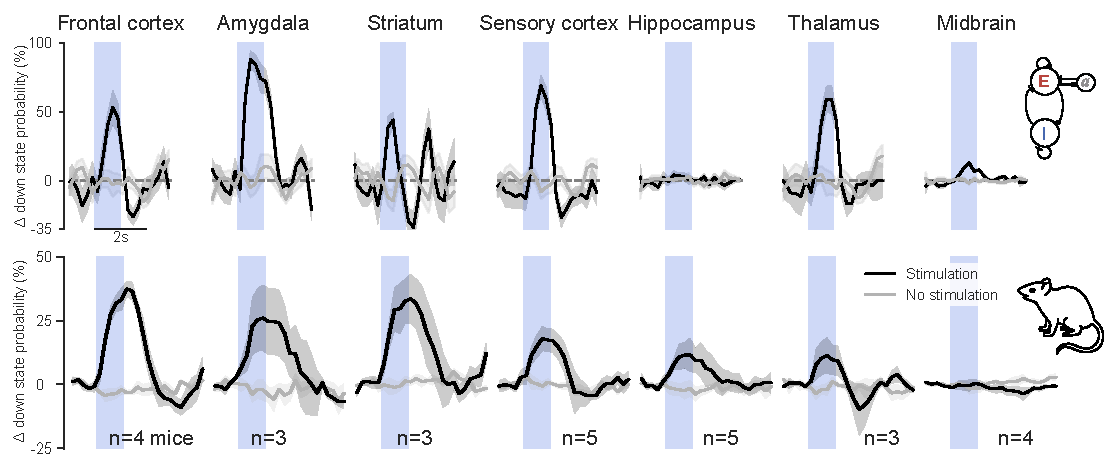
\includegraphics[width=0.9\textwidth]{img/Results/Figure2.pdf}
    \caption[Mouse vs. Model]{Mouse vs. Model. Serotonin stimulation induced a DOWN state in several regions. The top graph shows the model simulation, whereas the plot below demonstrates the findings from the recordings in mice. The y-axis shows the $\Delta$ DOWN state probability, which expresses the difference between the probability of a DOWN state occurring in stimulation sessions compared to sessions without stimulation (baseline).}
    \label{fig:downstate_repl}
\end{figure}
\\
\indent It was clearly visible that during optogenetic stimulation of the DRN in mice (area highlighted in light blue), the probability of a DOWN state increased between 25-50\% in the frontal cortex, amygdala and striatum, compared to the baseline activity, in which no stimulation was applied. The sensory cortex, hippocampus and thalamus showed an induced DOWN state too, though slightly less than the previously named areas (10-12\%). The midbrain seemed not to be affected by the serotonin modulation. With simulations using the proposed model very similar effects can be observed. In the frontal cortex, striatum, sensory cortex, and thalamus the probability increased by about 50\% in comparison with the baseline, and the amygdala showed an increase of even around 90\%. Note that the DOWN state probability in the striatum was not significantly different from zero (see \ref{fig:downstate_barplot}), whereas this was the case in the other named regions. The midbrain shows a slight increase (significantly different from the baseline mean) of the DOWN state probability, different to the recordings in mice, where the midbrain was not affected by the stimulation. What is interesting is that the hippocampus did not seem to be modulated by serotonin in the model, despite the observed 10\% increased probability of a DOWN state in the mouse brain. 
\\
\indent Some regions indicated the return of an UP state after the induced DOWN state in the mouse data, which are the frontal cortex, sensory cortex (though very marginal), and thalamus. In the model it is striking that the rebound UP state were slightly stronger expressed than in the mouse data; for example, the frontal cortex, sensory cortex and thalamus – overlapping with the affected regions in the experimental data -, and additionally in the striatum showed a rebound UP state. In the model, the rebound UP state was induced much faster than in the experimental condition. 


\begin{figure}[h]
    \centering
    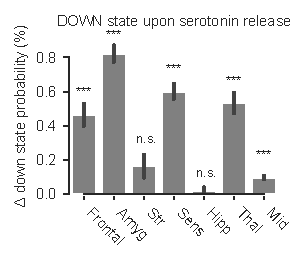
\includegraphics[width=0.45\textwidth]{img/Results/downstate_replicationS40_G[2].pdf}
    \caption[Effect of serotonin on DOWN state probability]{Effect of serotonin on DOWN state probability. Serotonin stimulation induces a DOWN state in several regions. Probability values between 0.5-1 seconds after the serotonin stimulation onset are included.}
    \label{fig:downstate_barplot}
\end{figure}

\indent What stands out is that the striatum showed strong fluctuations in the model simulations, in comparison to the other regions and in comparison to the measurements in mice.
In all recorded areas displaying a modulatory effect, there was a delay of 0.5 seconds in inducing a DOWN state. This delay was simulated by implementing the time course of the serotonergic response. 
Overall, the main effect of serotonin that was observed in the electrophysiological recordings of mice could be replicated with minimal exceptions.


\section{Effects of coupling strength\label{sec:effcoupling}}
\noindent
\indent In this section, the potential underlying mechanisms behind serotonergic modulation will be addressed. One aspect to consider is the connectivity between the regions in the network, which are crucial for inter-area communication. The coupling strength of those inter-area projections was modified by increasing the value of the parameter $G$ that defines the weight of the connectivity matrix $W$. If the effect of serotonin on the UP and DOWN dynamics acts in a direct way, inter-area coupling would not be required to replicate the induced DOWN state. Though, if the successful replication of the effect requires inter-area coupling, serotonin acts indirectly. This mechanism might vary across different areas. We applied serotonin stimulation and systematically increased the coupling strength $G$, to gain insights into the role of inter-area coupling in controlling the effect of serotonin stimulation. 
\\
\indent In an unconnected network (G=0), the probability of a DOWN state (compared to baseline activity) is dependent on the strength of the DRN projections targeting each area (see Figure \ref{fig:couplingstrength} A). Regions to which the DRN strongly connects, showed a strong DOWN state probability during serotonin stimulation.  The amygdala for example receives very strong connections from the DRN and therefore showed the highest modulatory effect of all of the regions in an unconnected network. The visual cortex, on the other hand, receives fewer projections from the DRN and is therefore almost not affected by the simulated serotonin stimulation. 
\\


\begin{figure}[h]
    \centering
    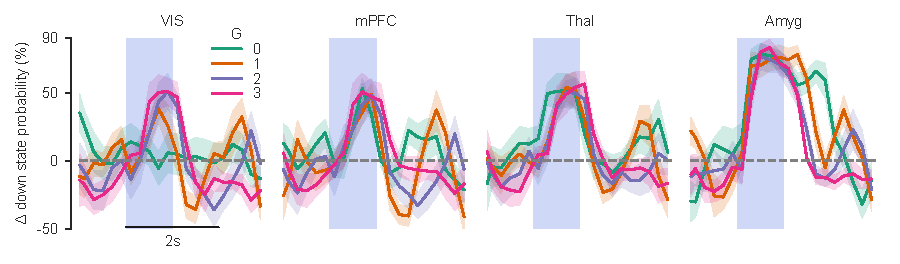
\includegraphics[width=0.9\textwidth]{img/Results/couplingstrength_trajectories_S40.pdf}
    \caption[Effect of coupling strength - Example traces]{Effect of coupling strength, demonstrated in example regions. The blue window indicates serotonin stimulation. The differently coloured graphs display different coupling strengths $G$ from $0-3$. The demonstrated example regions are the visual cortex (VIS), medial prefrontal cortex (mPFC), thalamus (Thal), and amygdala (Amyg).}
    \label{fig:couplingstrength_trajectories}
\end{figure}
\indent To investigate the effect of coupling strength, simulations with various coupling strengths were run ($G$ of $0-3$). Figure \ref{fig:couplingstrength_trajectories} demonstrates the resulting traces of DOWN state probability (each compared to the respective baseline) for the different coupling strength values in the visual cortex, medial prefrontal cortex, thalamus and amygdala. Modifying the coupling strength did not have the same effect in all areas. Whereas in the visual cortex, an increased coupling strength increased the DOWN state probability, the amygdala showed no big difference in DOWN state probability during serotonin stimulation for all G parameters. Additionally, it is noticeable that for $G=1$ in the visual cortex and the mPFC, the rebound UP state is distinctively pronounced.
In an unconnected network, the visual cortex was only slightly affected by serotonin stimulation (see Figure \ref{fig:couplingstrength} B). It was observed that with an increased coupling strength, the probability of a DOWN state increased in the visual cortex; it was around 50\% higher in the case of strong inter-area connections compared to no coupling.
\begin{figure}[h]
    \centering
    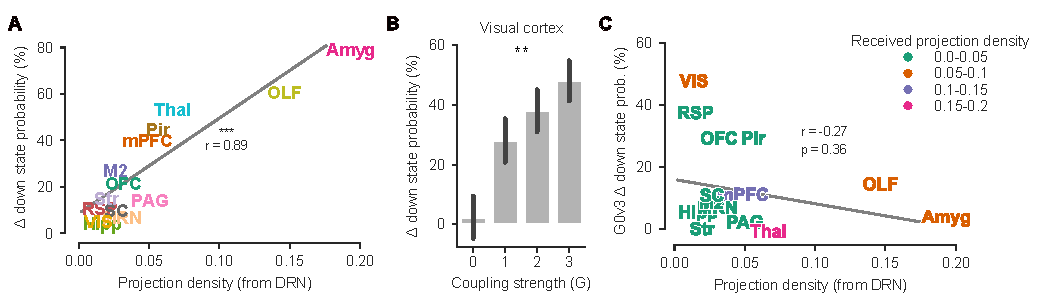
\includegraphics[width=0.9\textwidth]{img/Results/Figure3.pdf}
    \caption[Effect of coupling strength]{Effect of coupling strength. In all plots, DOWN state probabilities in a time window of 0.5-1 seconds post-stimulation were taken into account. A) In an unconnected network (G=0), the DRN projection density determines the strength of the effect of the modulation by serotonin. B) shows that the serotonin effect was elevated in the visual cortex for increased coupling strength (p<0.05). In C), the difference between the $\Delta$ DOWN state probability for a coupling strength G=0 and G=3 is displayed for every region. The colour codes describe the average projection densities that each area receives from all other areas, indicating how strongly the areas are affected by the changes in coupling strength.}
    \label{fig:couplingstrength}
\end{figure}
\\
\indent To uncover if this effect was similar for all of the regions, the difference between $\Delta$ DOWN state probabilities in an unconnected network and a strongly connected network were investigated (see Figure \ref{fig:couplingstrength} C). It turns out that whereas some areas were strongly affected by the change in coupling strength, others were not. The difference (G=0 vs G=3) was high for the visual cortex (p<0.05), but close to zero for the amygdala. Areas that did not show any UP-DOWN states were not affected by the increase in coupling strength either.
\\
\indent This could not be explained by the strength of DRN connectivity, as the negative correlation was non-significant (r=-0.27, p=0.36). The projection densities (obtained from the Allan Brain Atlas) describing the connection strength between the areas co-existing in this network vary (see legend in Figure \ref{fig:couplingstrength} C) and might affect how each area reacts to the coupling strength. The visual cortex receives relatively rich projections from other areas in the network, compared to the midbrain, striatum, thalamus, hippocampus, secondary motor cortex, and the remaining sensory regions. The thalamus showed, despite strong incoming inter-area projections, no enhanced serotonin effect for an increased coupling strength.   
\\
\indent Overall, the coupling strength affected serotonin's induced DOWN state in some but not all areas, which could not be explained by the strength of DRN projections. Neither was the density of inter-area projections of each area a determining factor. Therefore, it is interesting to examine the heterogeneous connectivity pattern of the regions in this network model.

\section{Heterogeneous connectivity}\label{sec:heterogconnect}
\noindent
\indent The previous results showed that the area specific connectivity pattern seems to be relevant for achieving an effect in some areas (see above in Section \ref{sec:effcoupling}). Using information about the projection densities between areas (from the Allen Brain Atlas) implemented the area specific connectivity in the model and improved its biological plausibility. To investigate the relevance and impact of this effort on the obtained results, the simulations using the 'realistic' connectivity values were compared to simulations using homogeneous connectivity values, in which the mean of the entire connectivity matrix was applied as a single weight for all inter-area projections. 


\begin{figure}[h]
    \centering
    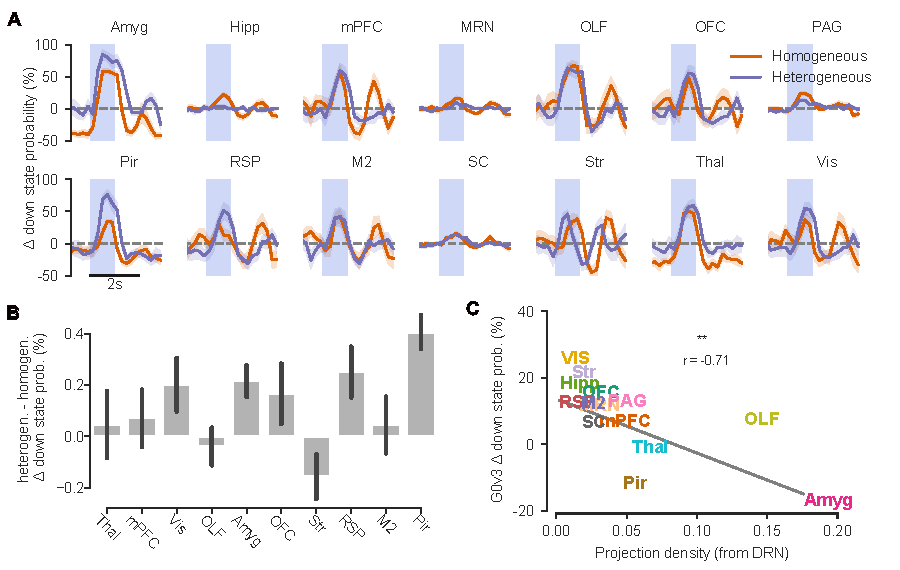
\includegraphics[width=0.95\textwidth]{img/Results/Figure5.pdf}
    \caption[Heterogeneous vs. homogeneous connectivity]{Heterogeneous vs. homogeneous connectivity. A) shows the trajectories of the DOWN state probability in homogeneous and heterogeneous connectivity compared to each of the baselines (coupling strength of $G=2$). B) demonstrates the difference between homogeneous and heterogeneous connectivity seen in A). Regions that did not show any UP and DOWN areas were excluded. The regions on the x-axis are sorted by incoming projection strength (from all other areas) from high density to low density. In C), the difference in $\Delta$ DOWN state probability between $G=0$ and $G=3$ in the homogeneous condition is plotted and correlated with the DRN projection strength of each area. B) and C) include data in a time window of 0.5-1 seconds post-stimulation.}
    \label{fig:heterogenconnect}
\end{figure}
In the homogeneous condition, a DOWN state was induced upon serotonin stimulation in all areas (Figure \ref{fig:heterogenconnect} A). In some regions, the heterogeneous coupling mechanism strengthened the effect of serotonin in comparison to the homogeneous coupling, whereas in other regions the effect was reduced (see Figure \ref{fig:heterogenconnect} B). The thalamus for example, which receives strong projections from the other areas in the heterogeneous condition, did not show a great difference between the homogeneous and heterogeneous condition. The piriform cortex, which is an area that does not receive many projections from other areas, showed an increased effect of serotonin is higher in the heterogeneous condition. Another example is the secondary motor cortex, whose response did not change a lot in the homogeneous coupling condition even though it also receives few projections in the heterogeneous condition. These different results in the homogeneous and heterogeneous conditions might be created due to the specific areas from which both regions receive input, as well as the strength of the DRN projections that both areas received. In the heterogeneous condition, the piriform cortex received projections mainly from the olfactory cortex, which was strongly targeted by the DRN. This connectivity profile was overwritten by the homogeneous connectivity value. 
\\
\indent In the homogeneous condition, there was a significant negative correlation (p<0.01) found between the projection density originating from the DRN and the difference in serotonin-induced DOWN state of a coupling strength of $G=0$ versus $G=3$ (see Figure \ref{fig:heterogenconnect} C). The increased coupling strength ($G=3$) had a higher influence on regions with low DRN projection densities. In some regions with a higher DRN connectivity, strong homogeneous coupling even reduced the DOWN state probability (e.g., in the amygdala).
\\
\indent In summary, heterogeneous inter-area coupling increased the efficacy by which of serotonin-induced DOWN states, compared to homogeneous coupling. Homogeneous coupling led to an evenly distributed effect across the regions.

\section{The mechanism of serotonin stimulation}
\noindent
\indent The mechanism used to simulate serotonin in the model plays a crucial role in replicating the effects observed in the experimental data. Here, the consequences of modifying the approach to serotonin stimulation within the model were investigated. Specifically, it was chosen to model serotonin stimulation as an inhibitory current targeting the E population ('$E-$'), as this increases the threshold for the E population to fire, making it likely to induce a transition from the UP to the DOWN state. It is also intuitive to consider the opposite operation of targeting the I population with an excitatory current ('$I+$'), as it may yield similar results. Figure \ref{fig:targetI} illustrates the outcomes of the simulation under this condition. 

\begin{figure}[h]
    \centering
    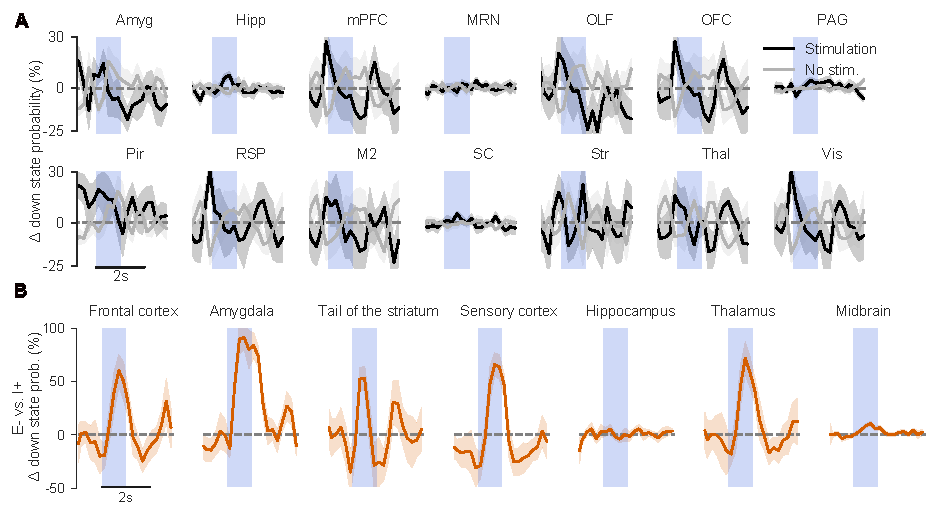
\includegraphics[width=1\textwidth]{img/Results/Figure4_1.pdf}
    \caption[Modelling serotonin by targeting the I population with an excitatory current]{Modelling serotonin by targeting the I population with an excitatory current. A) $\Delta$ DOWN state probability in all simulated brain regions. B) Difference between targeting E with an excitatory current and targeting I with an inhibitory current.}
    \label{fig:targetI}
\end{figure}


The graph reveals that, in many regions such as the Amygdala, cortical areas (OLF, OFC, M2, Vis, Pir, and RSP) and the striatum, a first spike of an induced DOWN state took place, followed by an UP state at around 1 second after stimulation onset. This is interesting since this is the opposite effect of what was observed when targeting the E population with an inhibitory current, as the main effect, the induced DOWN state could be observed around the same time as the UP state in this modified serotonin stimulation. Note, that the highest $\Delta$ DOWN state probability did not exceed 30\%, which is very low in comparison to the probabilities found when targeting population E with an inhibitory current (see Figure \ref{fig:downstate_repl}). In the somatosensory cortex as well as in the piriform cortex and thalamus, the initial DOWN state that occurred within the first 0.5 seconds after stimulation was longer and less 'spiky' that in the other regions named above. The serotonin stimulation acts gradually, therefore the current applied to I is rather weak at first. Nevertheless, the local circuit reacted to the weak current applied to the I population with an increased DOWN state probability. In turn, a stronger current had the opposite effect and let the system transition into an UP state. 
\\
\indent Figure \ref{fig:targetI} B shows the direct comparison of the two distinct mechanisms ('$E-$' and '$I+$'). If both mechanisms were to induce the same effect, it was expected to observe a line centred around 0. Though, it is visible that the clear DOWN state in all regions except the hippocampus and the midbrain could not be replicated by the $I+$ mechanism.


\begin{figure}[h]
    \centering
    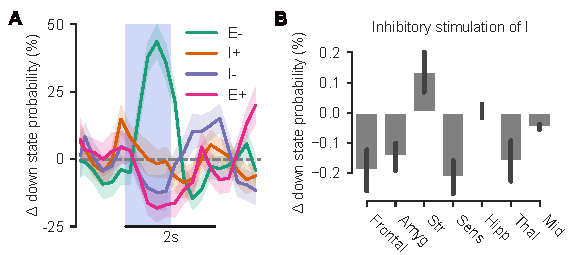
\includegraphics[width=0.8\textwidth]{img/Results/Figure4.pdf}
    \caption[Target mechanisms of serotonin stimulation]{Target mechanisms of serotonin stimulation. A) All four options of modelling serotonin stimulation, averaged over all regions in the network. The first letter in the legend description is the population targeted by serotonin, the sign after it indicates the charge direction of the current to that population. B) shows a more detailed view of the 'I-' simulation. Downstate probabilities in a time window of 0.5-1 seconds post-stimulation are taken into account.}
    \label{fig:targetI2}
\end{figure}
\indent To uncover the effects of other options for modelling serotonin stimulation, targeting the E population with an excitatory current ('$E+$') and targeting the I population with an inhibitory current were investigated ('$I-$'). The results of all four mechanisms ('$I+$', '$E-$', '$I-$', and '$E+$') are presented in Figure \ref{fig:targetI2} A. It is evident that only the '$E-$' implementation successfully reproduced a stable induction of a DOWN state during serotonin stimulation, followed by a somewhat less probable rebound UP state. As demonstrated previously, modelling the stimulation using the '$I+$' mechanism failed to replicate the desired effect. Notably, the '$E+$' and the '$I-$' mechanism led to the induction of an UP state with a probability of approximately 10-20\% compared to the baseline (note that the inverse of the DOWN state probability equals the probability of an UP state). Figure \ref{fig:targetI2} B shows that for the '$I-$' mechanism an UP state in frontal areas, amygdala, sensory areas and the thalamus was induced. Interestingly, a subtle induction of a DOWN state was observed in the striatum. This phenomenon could be attributed to the comparatively higher frequency of oscillations in the striatum relative to other areas.
\\
\indent The clear distinctions in the outcomes achieved by each mechanism highlight the complexity of the network model.

